\chapter{Zagrożenia współczesne i socjotechnika\index{socjotechnika}}
\newpage
\section{Ransomware}
Złośliwe oprogramowanie, które dosłownie „bierze nasze dane jako zakładników”.
\begin{itemize}
    \item Szyfruje pliki osobiste lub całkowicie blokuje dostęp do systemu (komputera, smartfona)
    \item Głównym celem jest wymuszenie okupu\index{okup} (często płatnego w kryptowalutach) w zamian za przywrócenie dostępu do danych
    \item Do infekcji dochodzi najczęściej poprzez nieostrożność użytkownika (np. kliknięcie w podejrzany załącznik mailowy – \textit{malspam\index{malspam}}, lub fałszywą reklamę – \textit{malvertising \index{malvertising}}) \cite{ransomware}
\end{itemize}
\begin{figure}[!h]
    \centering
    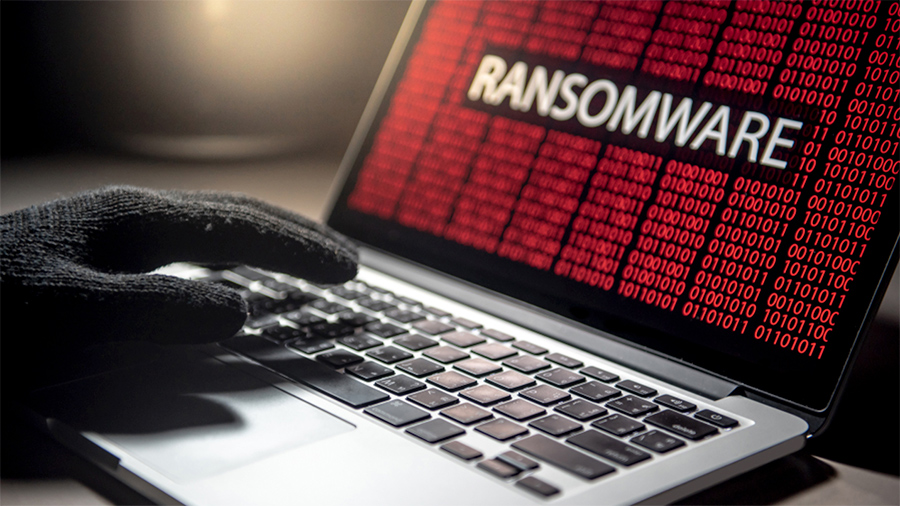
\includegraphics[width=1\linewidth]{ransomware.png}
    \caption{Wizualizacja ataku typu ransomware. \cite{grafiki}}
    \label{fig:ransomware}
\end{figure}
\newpage
\subsection{Przykład-WannaCry\index{WannaCry}}
\begin{figure}[!h]
    \centering
    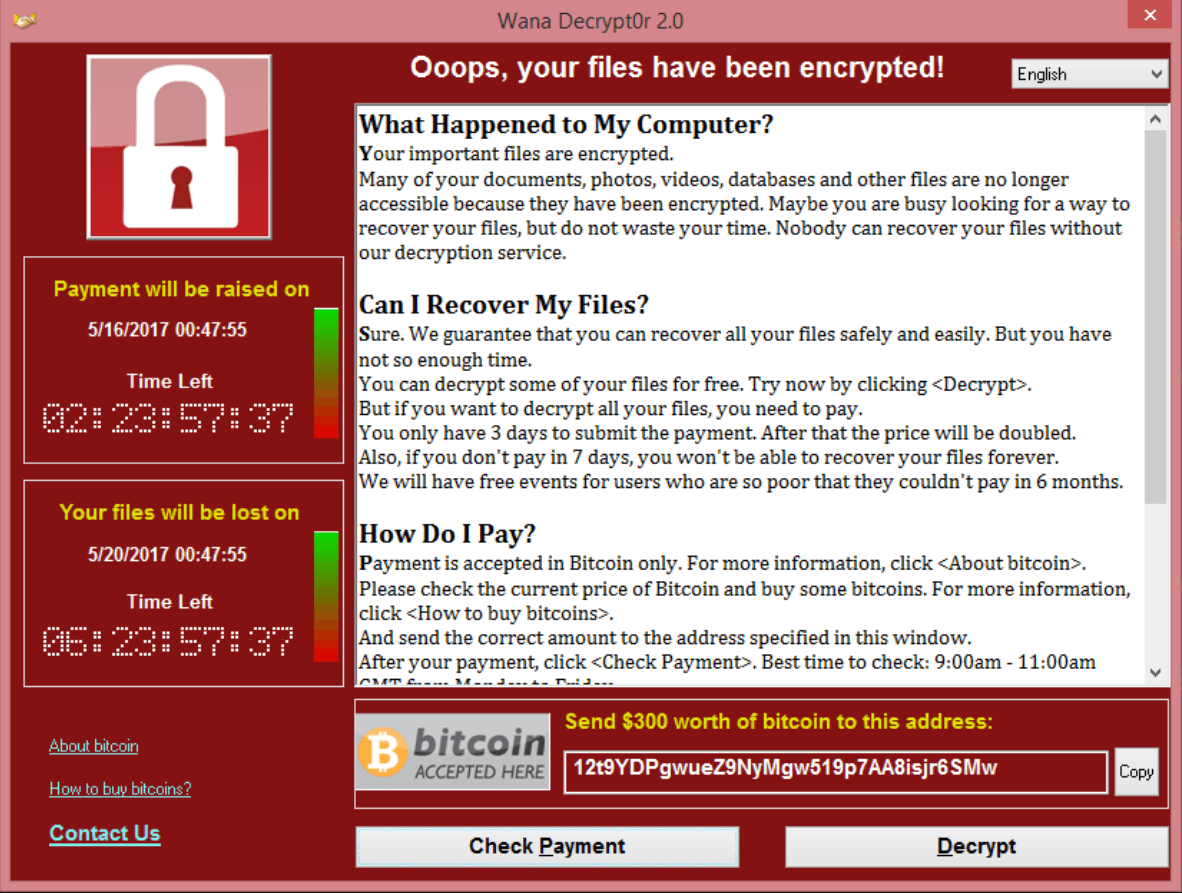
\includegraphics[width=1\linewidth]{Wannacry.png}
    \caption{Komunikat żądanie okupu z ataku WannaCry. \cite{grafiki}}
    \label{fig:WannaCry}
\end{figure}

\noindent Zgodnie z ilustracją \ref{fig:WannaCry}, użytkownik otrzymuje określoną ilość czasu na zapłatę. W przypadku \textbf{WannaCry} atak wykorzystywał lukę w systemach Windows o nazwie \texttt{EternalBlue}.

\begin{itemize}
    \item \textbf{Pochodzenie i twórca:} Nieznany (podejrzenia kierowane w stronę Korei Północnej)
    \item \textbf{Data ataku:} 12 maja 2017
    \item \textbf{Metoda ataku:} Ransomware (szyfrujące) + Robak (wykorzystanie luki „EternalBlue”)
    \item \textbf{Skutki infekcji:} Szyfrowanie\index{szyfrowanie} danych i żądanie okupu, paraliż ponad 230 tys. Komputerów
    \item \textbf{Zatrzymanie:} Odkrycie „wyłącznika awaryjnego” (kill switch) przez brytyjskiego badacza \cite{wannacry}
\end{itemize}
\newpage
\section{Trojan}
Złośliwe oprogramowanie, które podszywa się pod użyteczne i legalne programy.
\begin{itemize}
    \item Ukrywa swoje prawdziwe zamiary pod przykrywką przydatnej aplikacji, licząc na to, że użytkownik sam go zainstaluje.
    \item W przeciwieństwie do wirusów i robaków, trojany zazwyczaj nie replikują się samodzielnie i potrzebują interakcji użytkownika (np. uruchomienia pobranego pliku).
    \item Często służy jako furtka dla innych zagrożeń – kradnie dane (hasła, dane finansowe), szpieguje (\textit{spyware}) lub pobiera kolejne złośliwe programy, np. \textit{ransomware}. \cite{trojan}
\end{itemize}
\begin{figure}[!h]
    \centering
    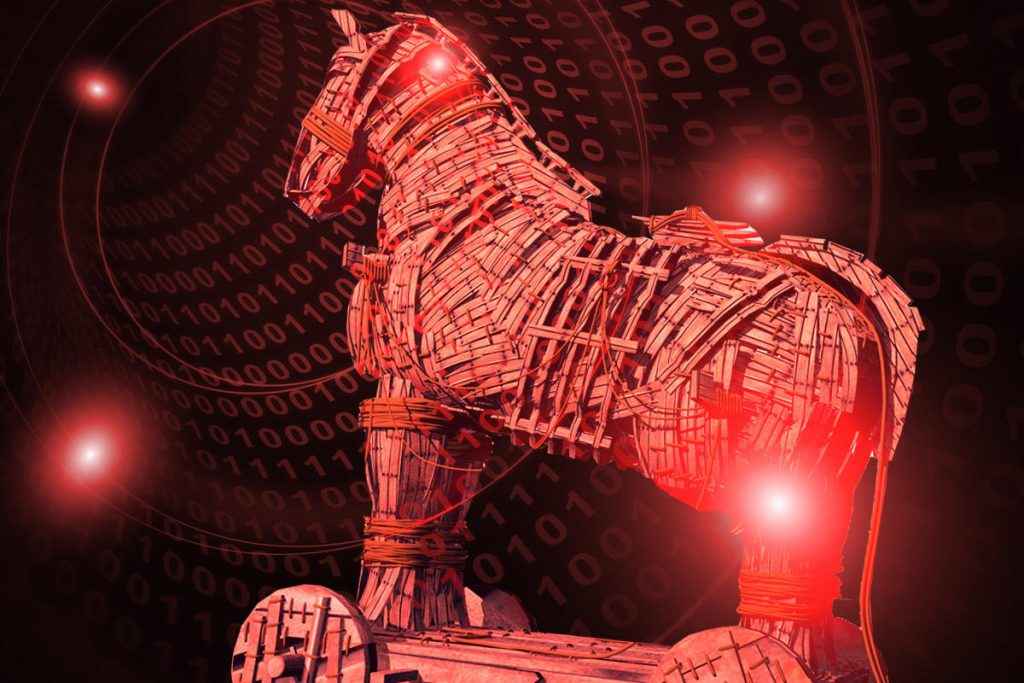
\includegraphics[width=1\linewidth]{Trojan.png}
    \caption{Wizualizacja konia trojańskiego jako metafory złośliwego oprogramowania. \cite{grafiki}}
    \label{fig:trojan}
\end{figure}
\newpage
\subsection{Przykład- Watykańczyk\index{Watykańczyk}}
\begin{itemize}
    \item \textbf{Pochodzenie:} Polska (ok. 2016 roku)
    \item \textbf{Typ:} Specyficzna forma złośliwego oprogramowania (tzw. joke program\index{joke program}) \cite{papiez}
    \item \textbf{Sposób działania:} Utrudniał korzystanie z komputera poprzez sekwencję zdarzeń.
    \item \textbf{Skutki infekcji:} Nie niszczył i nie kradł danych jego zadaniem było trollowanie użytkownika 
\end{itemize}
Film z demonstracją działania został opisany w Dodatku \ref{zal:watykanczyk}
\begin{figure}[!h]
        \centering
        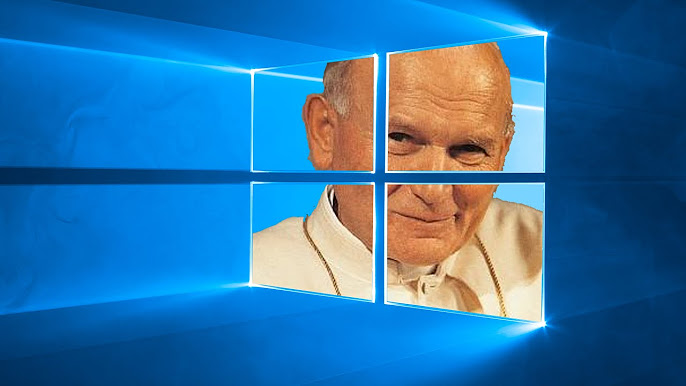
\includegraphics[width=1\linewidth]{papiez.png}
        \caption{Modyfikacja tapety systemu Windows charakterystyczna dla działania programu Watykańczyk. \cite{grafiki}}
        \label{fig:watykanczyk}
    \end{figure}
\newpage
\begin{figure}[!h]
        \centering
        
\includegraphics[width=1\linewidth]{dziekuje_za_uwage.png}
        \caption{Dziękuję za uwagę. \cite{grafiki}}
        \label{fig:slajd_końcowy}
    \end{figure}
    